Le choix de Windows Server 2003 Entreprise Edition s'est imposé pour l'installation de la maquette. Cette version intégrant toutes les fonctionnalités nécessaires à la mise en place d'un VPN aucune application tierce ne sera à priori requise.

Nous commencerons par détailler les différents services nécessaires au fonctionnement du VPN sur le serveur, ensuite nous verrons les méthodes de configuration d'un poste client et enfin nous effectuerons une synthèse des avantages et inconvénients de la solution Microsoft.

\subsubsection{Côté serveur : les services installés}

Dans cette section nous détaillerons tour à tour la configuration des nombreux services requis pour le bon fonctionnement du service VPN:
\begin{itemize}
	\item service DHCP.
	\item service DNS.
	\item Active Directory.
	\item routage et accès distant (VPN).
	\item autorité de certification (CA).
	\item IIS (requis pour l'authorité de certification)
\end{itemize}
~

% Remarque : Sous windows on ne parle pas de serveur mais de service. Tout les fonctionnalités de la machine (DNS, DHCP ou autre) sont référencés comme des services.


\paragraph{Caractéristiques de la machine}
~

Le serveur windows est installé sur un DELL PowerEdge 1300. Il est doté d'un processeur INTEL de type Pentium II cadencé à 348 Mhz, possède 512 Mo de mémoire vive ainsi qu'un disque dur de 9 Go. La machine est également équipée de trois cartes réseaux 100Mbps configurées comme suit :

\begin{figure}[H]
	\begin{center}
		\begin{tabular}{l|c|c}
		Référence & Réseau & Adresse IP \\
		\hline
		Realtek RTL 8139 Familly & réseau PROFS & 10.0.0.11/24 \\
		Realtek RTL 8139 Familly & réseau extérieur & 192.168.102.250/24 \\
		Fast Ethernet CNET PRO 200P & réseau STUDENTS & 192.168.0.11/24 \\
	\end{tabular}
	\end{center}
	\caption{Configuration des cartes réseaux}
	\label{IP_carte_reseau}
\end{figure}

\paragraph{Service DHCP}
~

Ce service est nécessaire pour l'attribution des adresses IP qui seront allouées à chaque client voulant se connecter. La configuration du service DHCP met en évidence les deux pools d'adresses nécessaires à l'adressage de chacun de nos réseaux internes :

\begin{figure}[H]
	\begin{center}
		\begin{tabular}{l|c|c}
			Caractéristique & Réseau PROFS & Réseau STUDENTS \\
			\hline
			Désignation Carte réseau & DHCP\_PROFS & DHCP\_STUDENTS \\
			Adresse IP Carte réseau & 10.0.0.11 & 192.168.0.11 \\
			Pool d'adresse & 10.0.2.100 à 10.0.2.254 & 192.168.2.100 à 192.168.2.254 \\
			Masque réseau & 255.255.255.0 & 255.255.255.0 \\
			Serveur DNS/routeur & 10.0.0.11 & 192.168.0.11 \\
			Nom du domaine DNS & wvpn.isima.fr & wvpn.isima.fr \\
		\end{tabular}
	\end{center}
	\caption{Caractéristiques du service DHCP}
	\label{service_DHCP}
\end{figure}

L'installation du service DHCP ne requiert aucune modification des options par défaut, et ne nécessite que d'indiquer qu'elles sont les cartes réseau à adresser. La figure \ref{Screen_client_dhcp} illustre cette configuration :

\begin{figure}[H]
	\begin{center}
	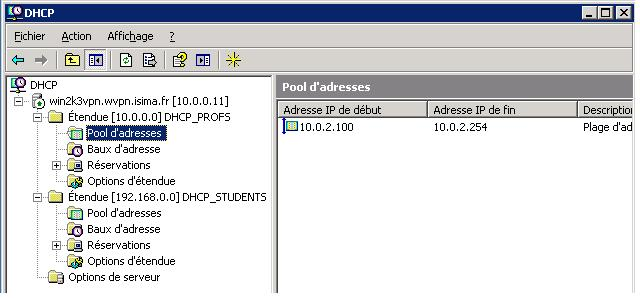
\includegraphics[width=\textwidth]{partie_2/screen_windows/dhcp.JPG}\\
	\end{center}
	\caption{Etendue DHCP du réseau professeurs}
	\label{Screen_client_dhcp}
\end{figure}
~

Il est à noter que sous Windows le service DHCP est attaché à une seule carte réseau qui répondra aux demandes des clients, ici la carte \verb|DHCP_PROFS|
% Cependant, le service DHCP s'attache à une seule carte réseau et non au deux. Dans la maquette, le service se lie avec la carte DHCP\_PROFS. Pour illustrer ces propos, voici un screenshot du service DHCP.

% On remarque que bien que la présence des deux étendues et que la carte DHCP\_PROFS (10.0.0.11) s'attache au service DHCP.
% ~\


% Voyons à présent la configuration du service DNS.

\paragraph{Service DNS}
~

En préliminaire à l'installation de Active Directory, un service DNS est requis. Les caractéristiques de ce dernier sont les suivantes :
\begin{itemize}
	\item Nom de la machine : win2k3vpn.
	\item Nom de domaine : wvpn.isima.fr.
	\item Type de zone : zone principale.
\end{itemize}
~

% Il est à remarquer que lors de l'installation du service, nous avons décider d'incorporer la zone de recherche inversée. Le serveur windows étant composé de trois cartes réseaux, il y a trois zones.

% Afin de vérifier que le service DNS est bien configurer, la commande NSLOOKUP nous permet de tester le DNS. 
% L'illustration suivante montre la résolution DNS est correcte.
% 
% \begin{figure}[H]
% 	\begin{center}
% 		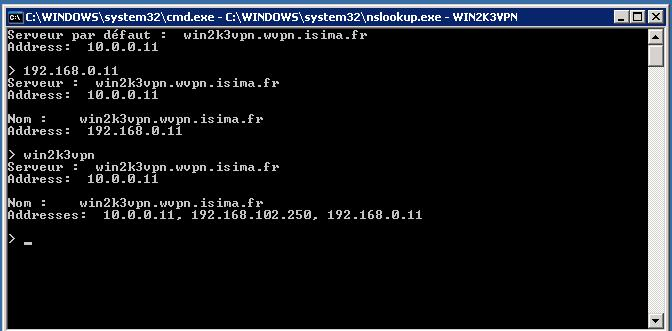
\includegraphics[width=\textwidth]{partie_2/screen_windows/nslookup.JPG}\\
% 	\end{center}
% 	\caption{Résolution DNS}
% 	\label{NSLOOKUP}
% \end{figure}

Tout comme pour le service DHCP, le service DNS est attaché à une seule carte réseau.

% Intéressons nous à présent à la configuration de l'Active Directory.

\paragraph{Active Directory}
~

Ce service fournit le support d'un annuaire permettant l'identification des clients. Notre VPN proposant deux accès distincts, deux groupes doivent être créés : un groupe STUDENTS et un groupe PROFS. Lors de la configuration d'un nouvel utilisateur, celui-ci doit être ajouté dans l'un de ces groupes et doit être explicitement autorisé à pouvoir se connecter :

\begin{figure}[H]
	\begin{center}
		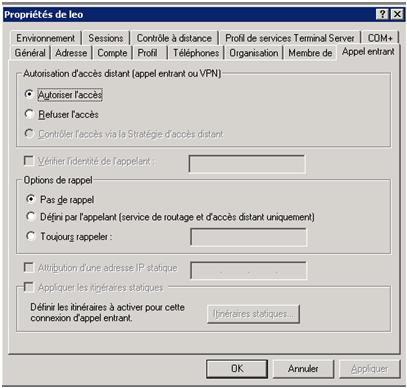
\includegraphics[width=0.50\textwidth]{partie_2/screen_windows/vpn.JPG}\\
	\end{center}
	\caption{Autorisation d'un utilisateur à se connecter au VPN}
	\label{VPN_AUTORISATION}
\end{figure}

La stratégie de groupe (GPO) a été laissée à sa configuration par défaut.

% Une fois les services de base installé, voyons à présent la configuration du service de \textit{Routage et accès distant} .

\paragraph{Routage et accès distant}
~\

Le service routage et accès distant est le service qui va nous permettre de monter un tunnel sécurisé. Lors de son installation, l'administrateur doit choisir l'option ``routage pour réseaux locaux uniquement'' ainsi que l'option ``serveur d'accès distant''. Une fois le service installé, il faut configurer les options de sécurité qui sont propre au serveur (un clic droit sur le nom du serveur permet de modifier les propriétés) pour correspondre à la manière dont les utilisateurs s'identifient. Le service propose deux choix : identification par l'annuaire et identification via un serveur RADIUS.

\begin{figure}[H]
	\begin{center}
		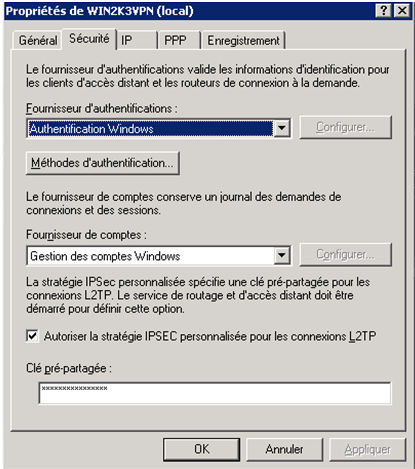
\includegraphics[width=0.50\textwidth]{partie_2/screen_windows/secu_vpn.PNG}\\
	\end{center}
	\caption{Choix de la méthode d'identification}
	\label{VPN_AUTHENTIFICATION}
\end{figure}

Nous avons testé la maquette en activant l'identification via un serveur RADIUS afin de pouvoir récupérer l'annuaire de l'ISIMA (comme présenté pour la configuration du routeur CICSO en 2.3.2.\ref{CONFIG_RADIUS} page \pageref{CONFIG_RADIUS}), mais cela n'a jamais fonctionné comme escompté. Afin de travailler avec une maquette fonctionnelle nous avons dû rétablir le mode d'authentification via annuaire local.

Dans l'onglet IP, il faut configurer la manière dont le service va attribuer les adresses IP aux clients : soit via le service DHCP (méthode la plus flexible, que nous avons retenue), soit en définissant manuellement une plage statique à adresser. L'option ``carte'' correspond à la carte réseau qui repondra aux demandes des clients.

\begin{figure}[H]
	\begin{center}
		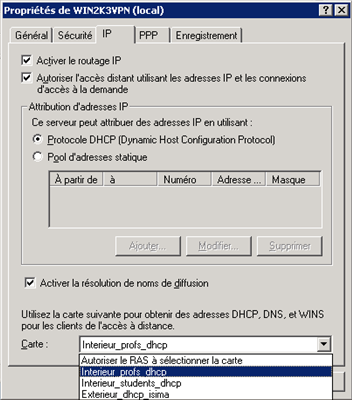
\includegraphics[width=0.50\textwidth]{partie_2/screen_windows/choix_carte.PNG}\\
	\end{center}
	\caption{Configuration du routage IP}
	\label{VPN_CARTE_ECOUTE}
\end{figure}

La problème est le même que pour les services DHCP et DNS : le service d'accès distant s'attache à une seule carte réseau.
% En naviguant dans les différentes options, on se rend rapidement compte que le service d'accès distant se lie avec une seule carte réseau. C'est la grande limitation. Il n'est pas possible que les deux cartes réseaux destinés pour le traffic interne redirige les différents flux réseaux.
L'aspect sécurité est géré par l'intermédiaire des stratégies d'accès distant. Il nous en falait une dont voici les spécifications :

\begin{itemize}
 	\item Appartenance à un groupe : PROFS ou STUDENTS
	\item Type d'authentification : MS-CHAP V2
	\item Spécification du type de connexion : VPN
\end{itemize}
~

La stratégie d'accès distant permet de contrôler finement quelles sont les conditions que doit remplir un utilisateur pour pouvoir se connecter, par exemple en définissant une plage horraire de connexion, etc. L'authentification utilise le protocole propriétaire Ms-Chap v2 qui permet une authentification mutuelle du client et du serveur. L'inconvénient de ce protocole est qu'il laisse passer le login du client en clair sur le réseau, mais les mots de passes sont bien sûr hashés.

\begin{figure}[H]
	\begin{center}
		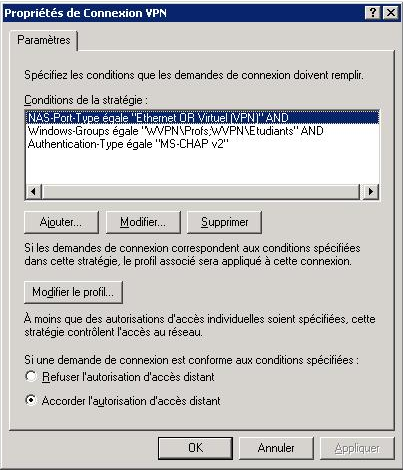
\includegraphics[width=0.50\textwidth]{partie_2/screen_windows/strat.png}\\
	\end{center}
	\caption{Stratégie d'accès distant}
	\label{VPN_STRAT}
\end{figure}

% Dans la stratégie d'accès on peut rajouter un paramètre sur la date. En effet, on le paramétrant, on peut définir une plage horaire où l'utilisateur ne pourra pas se connecter.

% Concernant le tyoe d'authentification, on utilise le protocole MS-CHAP V2 qui est un protocole propriétaire de Miscrosoft. En complement de cela, le serveur VPN fait un challenge de type MD5 afin d'authentifier le client.

% Le protocole MS-CHAP V2 utilise une authentification mutuelle. Cela permet au serveur d'authentification et à la machine distante de vérifier leurs identités respectives. L'inconvenient de cette méthode est que le login du client passe en clair sur le réseau. En sniffant la connexion par l'intermédiare de Wireshark, nous nous sommes rendu compte de cela. Par contre, le challenge MD5, et les mots de passe sont chiffrés.

% Afin d'améliorer la sécurité, nous avons décider de mettre en place une autorité de certification.

\paragraph{Autorité de certification}
\label{autorité_certification}~

La sécurité de la solution n'est pas complète sans une identification via certificats, nous allons donc configurer une autorité de certification sur le serveur. Cette autorité va notamment nous permettre de délivrer des certificats signés qui nous seront utile pour la solution Microsoft, mais aussi lors de la configuration du routeur CISCO. L'autorité racine aura comme nom commun ISIMA et les certificats seront valides un an. L'ensemble correspond à la configuration du service Windows 2003 SCEP. D'un point de vue technique, l'autorité de certification utilise l'algorithme de hashage SHA-1 pour la signature, et un chiffrement de clefs de longueur 2048 bits par l'algorithme RSA.

Pour effectuer une demande de certificat, les clients doivent se connecter sur l'URL suivante : \verb|http://192.168.102.250/certsrv|. Deux types de certificats sont proposés : WEB ou MESSAGERIE. L'interface de l'autorité de certification permet de répondre aux demanded de certificats en choisissant d'accepter ou non de les délivrer. Si la demande est validée, l'utilisateur doit se connecter à nouveau sur le site WEB afin d'installer le certificat sur sa machine.

Malheureusement, après plusieurs essais infructueux nous constatons que le système de certificats ne nous permet plus de se connecter au VPN. Le problème se situe probablement dans l'écriture des demandes de certificats mais nous ne sommes pas parvenus le résoudre, et cela est dommageable pour le niveau de sécurité de la solution.

\subsubsection{Configuration du client}
\label{label_client_windows}

L'un des avantages majeurs de la solution Windows est que le client VPN est déjà intégrer dans le système d'exploitation de Microsoft. L'un des inconvénients majeurs de la solution Windows est que malgré touts nos efforts nous ne sommes jamais parvenus à nous connecter au VPN Windows depuis un client Linux. Cette section présente les différentes étapes nécessaires à la création d'une connexion VPN sous Windows, et débute par la configuration d'une nouvelle connexion de type entreprise :

\begin{figure}[H]
	\begin{minipage}{0.5\textwidth}
		\begin{flushleft} \large
			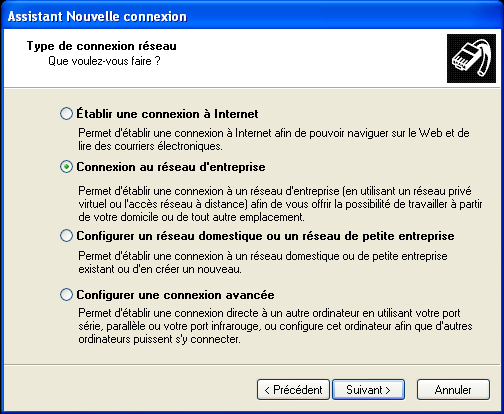
\includegraphics[width=0.95\textwidth]{partie_2/screen_windows/etape1.PNG}\\
		\end{flushleft}
	\end{minipage}
	\begin{minipage}{0.49\textwidth}
		\begin{flushright} \large
			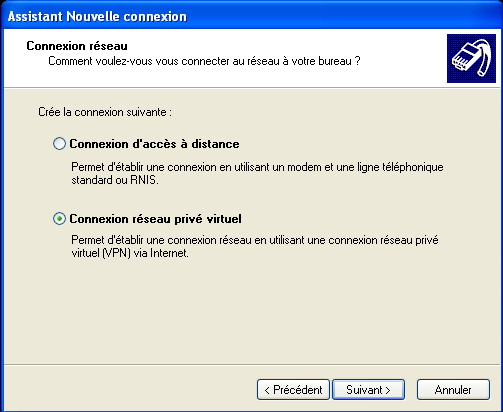
\includegraphics[width=0.95\textwidth]{partie_2/screen_windows/etape2.PNG}\\
		\end{flushright}
	\end{minipage}
	\caption{1ère étape de la configuration d'une nouvelle connexion}
	\label{VPN_ETAPE1}
\end{figure}
~\

La 2ème étape consiste à nommer la connexion et à désactiver le mécanisme de connexion initiale automatique :

\begin{figure}[H]
	\begin{minipage}{0.5\textwidth}
		\begin{flushleft} \large
			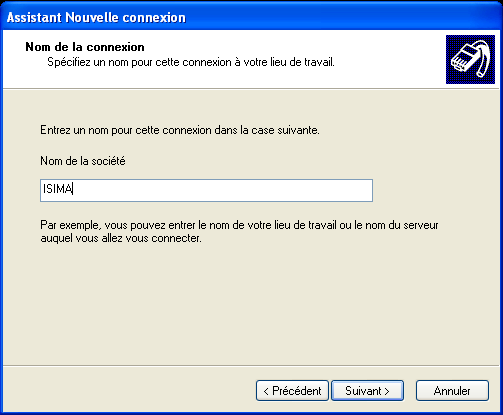
\includegraphics[width=0.95\textwidth]{partie_2/screen_windows/etape3.PNG}\\
		\end{flushleft}
	\end{minipage}
	\begin{minipage}{0.49\textwidth}
		\begin{flushright} \large
			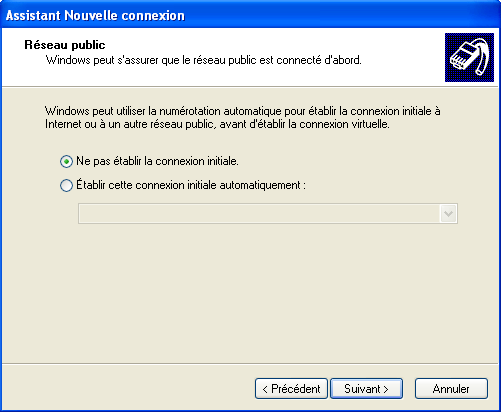
\includegraphics[width=0.95\textwidth]{partie_2/screen_windows/etape4.PNG}\\
		\end{flushright}
	\end{minipage}
	\caption{2ème étape de la configuration d'une nouvelle connexion}
	\label{VPN_ETAPE2}
\end{figure}
~\


La dernière étape permet de spécifier l'adresse IP du serveur distant : %. L'utilisateur pourra pour augmenter la sécurité utiliser une carte à puce pour s'authentifier.

\begin{figure}[H]
	\begin{minipage}{0.5\textwidth}
		\begin{flushleft} \large
			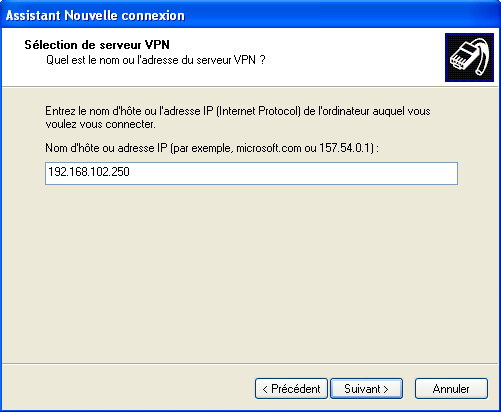
\includegraphics[width=0.95\textwidth]{partie_2/screen_windows/etape5.PNG}\\
		\end{flushleft}
	\end{minipage}
	\begin{minipage}{0.49\textwidth}
		\begin{flushright} \large
			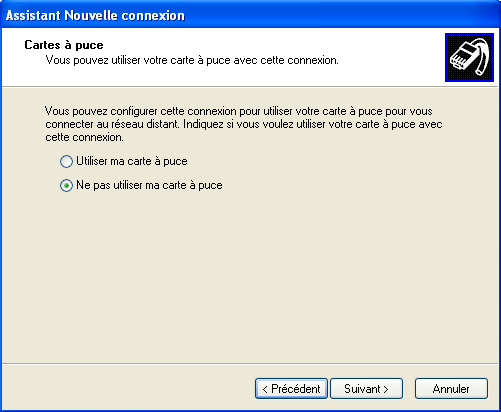
\includegraphics[width=0.95\textwidth]{partie_2/screen_windows/etape6.PNG}\\
		\end{flushright}
	\end{minipage}
	\caption{3ème étape de la configuration d'une nouvelle connexion}
	\label{VPN_ETAPE3}
\end{figure}

Ceci achève la configuration de la nouvelle connexion, les paramètres de sécurité du client ont été laissés aux valeurs par défaut. Lorsqu'il tentera de se connecter, l'utilisateur devra entrer ses identifiant et mot de passe comme définis dans l'Active Directory. La figure \ref{VPN_ETAPE7} présente l'état de la connexion après authentification : le VPN utilise le protocole PPTP, nous avons reçu l'adresse IP 10.0.2.106, authentification Ms-Chap v2, chiffrement MPPe 128 bits.

\begin{figure}[H]
	\begin{center}
		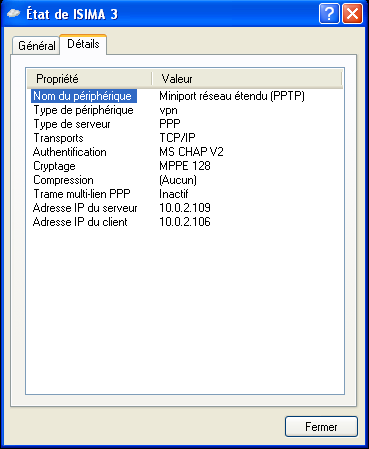
\includegraphics[width=0.50\textwidth]{partie_2/screen_windows/etape7.PNG}\\
	\end{center}
	\caption{Informations d'état de la connexion}
	\label{VPN_ETAPE7}
\end{figure}

% Cette image nous montre des informations importantes sur la nature du VPN. Tout d'abord, elle nous informe le protocole qu'elle utilise. Ici on utilise PPTP. Ensuite, le client nous donne le type de connexion : VPN ainsi que sa nouvelle adresse IP : 10.0.2.106
% Du point de vue sécurité, l'authentification se fait par l'intermédiaire de MS-CHAP V2 et le chiffrement par le protocole MPPE.

% MPPE est le protocole de chiffrement de Microsoft. Il se base l'algorithme RSA RC4. MPPE supporte trois tailles de clés : 40 bits, 56 bits et 128 bits.

Une remarque sur le chiffrement MPPe : Windows 2000 ne permet pas l'utilisation de clefs de longueur supérieure à 40 bits. Il est possible de permettre l'utilisation de clefs plus faibles que 128 bits sur le serveur, afin de permettre à ces clients de se connecter, mais ce n'est pas recommandé.
% Il est à noter que Windows 2000 ne permet pas l'utilisation de clefs de longueur supérieure à 40 bits. Il ne faut pas oublier d'activer sur le serveur VPN les différents tailles des clés sans quoi la connexion est refusée. 

\begin{figure}[H]
	\begin{center}
		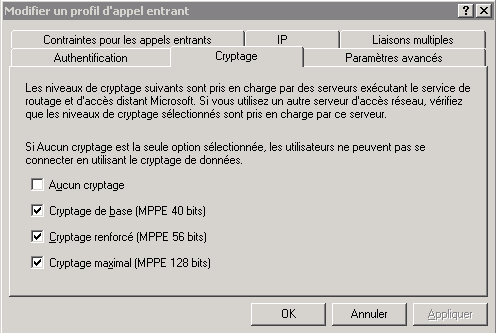
\includegraphics[width=0.50\textwidth]{partie_2/screen_windows/cryptage.PNG}\\
	\end{center}
	\caption{Cryptage MPPE}
	\label{VPN_CRYPTAGE}
\end{figure}


\subsubsection{Bilan et limites de la solution}

Microsoft propose une solution VPN à la fois intéressante et facile à mettre en place (côté serveur comme côté client), mais demeure vraiment destinée à de petites structures. Dans le cas de l'ISIMA, la structure du réseau est plus complexe, avec la séparation des réseaux professeurs et étudiants.

L'inconvénient majeur de Windows Server est que chaque service doit se lier avec une seule carte réseau. Il est donc impossible de dissocier le trafic réseau sur des deux cartes, ce qui ne respecte pas le cachier des charges du projet. Une solution envisageable serait de virtualiser un serveur Windows 2003 et de lier les cartes réseau virtuelles aux cartes réseaux physiques de la machine. Rappelons également que côté client nous n'avons pas réussi à nous connecter depuis une une machine Linux à cause d'une mauvaise implémentation du protocole PPTP.

La récupération des identifiants et mots de passe depuis l'annuaire de l'ISIMA n'a pas pu être effectuée et nous avons choisi de ne pas tenter d'interfacer notre maquette avec le réseau de l'école. Comme nous l'avons expliqué, le service VPN est attaché à une seule carte réseau, et ceci nous empêche de savoir quel type d'utilisateur est connecté (professeur ou étudiant). La procédure à suivre serait d'intégrer le serveur VPN Windows sur le domaine de l'ISIMA et de lancer une réplication de la base Active Directory.

Nous avons également suivi une autre piste pour tenter de s'interfacer avec la base NIS de l'ISIMA. Microsoft propose une suite d'outil \verb|Windows Service for UNIX| téléchargeable directement depuis leur site. Cette suite propose d'intégrer à Windows des commandes et services généralement spécifiques aux systèmes UNIX, parmis lesquels un client NIS. Une amélioration possible de la maquette serait de récupérer les informations utilisateurs de l'ISIMA via ces outils : l'interopérabilité serait alors complète.

L'absence de certificats signés pour l'authentification des pairs pose un réel probléme de sécurité. De plus bien que les mots de passes clients soient hashés, les identifiants et le nom d'hôte de la machine circulent en clair sur le réseau au cours de la phase d'authentification. La figure \ref{VPN_CONNEXION} illustre ce problème :

\begin{figure}[H]
	\begin{center}
		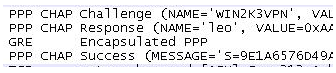
\includegraphics[width=0.5\textwidth]{partie_2/screen_windows/connexion.png}\\
	\end{center}
	\caption{Trace d'une connexion}
	\label{VPN_CONNEXION}
\end{figure}


% Par rapport à l'autorité de certifications, nous avons été capable de générer des certificats et les installer sur les machines tests. Par contre, la connexion avec le serveur VPN n'a pas pu s'établir. A l'heure actuel nous ne savons toujours pas d'où provient le problème. Nous soupçonnons un problème de communication entre l'autorité de certification et la machine test.

% Après avoir expliquer la configuration du serveur Windows 2003 et ses limitations, intéressons nous à la solution VPN sous Linux avec le logiciel OpenVPN.

En conclusion, la solution Microsoft bien que simple à mettre en place demeure incomplète, ne répond pas à notre cahier des charges en termes de sécurité et n'est pas multiplates-formes.
